\documentclass[showkeys,preprint]{revtex4-2}
%\documentclass[showkeys,preprint]{article}
\usepackage[utf8]{inputenc}
\usepackage{natbib}
\usepackage{graphicx}
\usepackage{amsmath}
\usepackage{lipsum}

\begin{document}
\title{A Hamiltonian theory for whistler chorus wave in the magnetosphere}
\author{Jiangshan Zheng}
\author{Ge Wang}
\author{Bo Li}
\affiliation{School of Physics, Beihang University, Beijing, 100191, China}
\date{\today}
\begin{abstract}
In this paper, we develop a novel Hamiltonian theory for the nonlinear resonant interactions between the energetic electrons and chorus wave in the magnetosphere.
Our theory studies the dynamics of the deeply trapped resonant electrons and the slowly varying coherent wave envelope in the reference frames moving with the local resonance.
We construct a new canonical transformation to separates the motion scales, and the Hamiltonian of the resonant particle is transformed to those on each local reference frames.
The Vlasov equation of the local distribution function is readily given and coupled with the slowly varying envelope equation derived from the Ampere's law self-consistently.
We further discuss the onset situation, i.e., the early chirping stage with small frequency variation, where we set the reference frame with time independent velocity at resonance of the linear most unstable wave to simplify the theoretic descriptions. 
We also consider the adiabatic regime and the water bag approximation for the evolution of resonant phase space structure and show its validation through a novel numerical simulation based on our scale separated theory.
Our theory and the corresponding numerical method are able to provide high resolution in phase space with affordable computation cost, which is urgently required to reveal the underlying physics of the nonlinear frequency chirping problem.
\end{abstract}
\maketitle

\section{Introduction}
\label{sec:intro}
Whistler-mode chorus is a special electromagnetic emission in whistler range of frequency, frequently observed in the planetary magnetosphere \cite{helliwell1965whistlers,burtis_magnetospheric_1976,tsurutani_postmidnight_1974}, and recently studied in the laboratory plasmas \cite{vancompernolle2015}.
The formation and evolution of chorus wave is related with the energy transference between wave and energetic electrons.
It plays a key role in particle acceleration processes in the radiation belt \cite{horne_wave_2005,thorne_rapid_2013,reeves_electron_2013} and pulsating and diffuse aurora in the atmosphere \cite{nishimura_identifying_2010,kasahara_pulsating_2018,thorne_scattering_2010}, which have received a significant research interest, such as in the studies of the superradiance in free-electron lasers \cite{zonca_nonlinear_2021, soto-chavez2012}.   

The physics of the chorus wave in essence are the nonlinear wave-particle interactions \cite{oneil1971,oneil1972} between the resonant trapped electrons and the whistler waves \cite{omura_theory_2008, an2019}. 
The similar nonlinear wave-particle interactions, such as the Alfv\'en wave instabilities \cite{chen2016,wang2018,wang2012,wang2012a} and energetic-particle-driven geodesic acoustic modes \cite{wang2013}, have been studies extensively in the fusion related plasma.
Such instabilities also involve the mode frequency sweeping and lead to premature ejection of alpha particles that deteriorate plasma confinement \cite{fasoli2007}.
The dynamics of nonlinear resonant particle can be modeled by Berk-Brizman (BB) model \cite{berk1990,berk1990a,berk1990b,berk1996,berk1997,berk1999}, which is a general theoretic model based on the bump-on-tail (BOT) paradigm. 
The original version and the advanced versions \cite{lilley2009,lilley2014a,vann2007,hezaveh2021,hezaveh2017,breizman2010,hezaveh2020} focus on the uniform regime, where the wave is treated as stationary with fixed wave number $k$. 
The spontaneous hole and clump structure and their evolution in the phase space were revealed and well explains the frequency chirping of the excited wave.
For the chorus wave case, the phase space behavior of the resonant electrons also plays an important role for the  chirping behavior.
It has been long time discussed \cite{sudan_theory_1971,vomvoridis_theory_1982,dysthe_studies_1971,nunn_self-consistent_1974,omura1991} and quantitatively explains the frequency chirping rate and nonlinear wave growth of chorus wave at various locations along the magnetic field \cite{tao_theoretical_2020,omura_nonlinear_2021,zonca_nonlinear_2021,zonca2022}.

However, although the BB model for the BOT paradigm was applied to study the chorus chirping problem \cite{soto-chavez2014}, a key feature for the chorus wave in the planetary magnetosphere is the involved inhomogeneous magnetic field. 
It was first noticed by Helliwell in his kinematic theory of the ``consistent-wave'' concept in the 1960s \cite{helliwell_theory_1967}.
It elucidates the change of chirping rate with respect to magnetic field inhomogeneity.
In more recent studies \cite{wu_controlling_2020,fujiwara2023}, it is found that the frequency chirping behavior can be controlled by changing the magnetic field configuration. Both downward chirping and bi-direction chirping were reproduced.
And a phenomenological chirping model called Trap-Release-Amplify (TaRA) model \cite{tao_trap-release-amplify_2021} was proposed and explained how frequency chirping occurs and why chirping direction with respect to the sign of magnetic field gradient.
Although the model has successfully explained chirping behavior in planetary magnetosphere, including that on Mars \cite{teng2023}, it raises the intriguing question of how rapidly varying chirping elements and resonant electrons are influenced by the background magnetic field's inhomogeneity.
This is despite the fact that the scale of the field's inhomogeneity is significantly larger than the characteristic scales of rapid changes and fine structure.
Besides, numerical simulations of artificially triggered emissions show different mechanism for the formation of chorus wave \cite{nogi2022,nogi2023}. 
The wave source moves with a velocity that is a combination of the group velocity and resonance velocity, rather than the velocity alone. This suggests that the chirping may not be emitted by the released particle.

Anyhow, in current theoretical and numerical studies, many questions still remain regarding the fine structures of the chorus observed in the magnetosphere. \cite{zhang2021}. 
The chirping mechanism with respect to the nonlinear wave particle interaction and the fine structures of the chorus wave are also addressed in the recently studies \cite{omura_nonlinear_2021,gao2014a,li2019b}.
Additional information about the particle dynamics and wave evolution, such as high resolution phase-space structure, fine wave number and frequency results, are still desired in additional to the satellite observations.
The numerical modelings are favorable for solving such issue \cite{katoh_computer_2007,vhscode,xiao2015,xiao2020explicit,xie2022,tao_numerical_2014,chen2015a}
However, due to introduce background magnetic field inhomogeneity, the simulation for the chorus wave is essentially multiscale.
Finding an appropriate method to separate the scales of resonant particles is a complex task because of the intricate interactions between waves and particles along the inhomogeneous magnetic field. 
Challenges and the need have spurred the development of a new theoretical and numerical model.

In this paper, we go over the dynamics of resonant electrons and the evolution of whistler wave in Earth inner magnetosphere.
The key feature in our theory is the scale separation of electron motion to the slowly one along the magnetic field and the fast wave interaction. 
To do so, we build a Hamiltonian theory in the reference frame moving with local resonance.
We divide the continuous spatial domain of the single magnetic field line into a group of cells representing a group of local reference.
By expanding the phase of the wave and the resonance electrons, a canonical Hamiltonian on the cell is constructed which naturally separated the fast and slowly varying motion of resonant electrons.
The canonical motion equations are then derived, which governs the dynamics of resonant electrons. 
The evolution of whistler-mode wave is determined by the Ampere equation, in which the wave is expressed in its eikonal form, thus, the frequency and wave number can be given directly and accurately.
With the established theory, we then discuss the onset stage of the chirping, which gives a more brief form for the local Hamiltonian. 
In the onset condition, the frequency of the wave is assumed to be time independent, and we show an integral of motion for the trapped electrons under resonant interactions.
We then show the adiabatic regime of the resonant electron phase space behavior, and verified adiabatic approximation from simulation based on our theory.


We organize our paper as follows. In section~\ref{sec:theory}, we present the Hamiltonian theory and derive the Vlasov equation for the resonant particle distribution, and the wave equation for the slowly varying wave envelope.
In section~\ref{sec:dis}, 
% and give the chirping rate at typical parameters.  
Finally, the summary is presented in section~\ref{sec:conc}.


\section{Hamiltonian Theory in local resonance frame}
\label{sec:theory}
%Hamiltonian 
%Given the Hamiltonian and wave form (original)
%PART I: THE WAVE
Consider an electron with mass $m_e$ gyrating in a weakly inhomogeneous magnetic field.
It interacts with a  narrowband traveling wave propagating along the magnetic field line. 
%with varying phase $\phi_q$.
The wave vector potential can be represented in a Fourier integral
\begin{equation}\label{eq.def_A}
    \mathbf{A}(s,t) =  \int_{-\infty}^{\infty}\mathrm{d} q~ \mathbf{A}\left(q,t\right) \exp(\imath\phi_{q})~,
\end{equation}
where 
\begin{equation}
    \phi_q \equiv \int^t \omega(q, \tau)d\tau - q s~
\end{equation}
% $\phi_q \equiv \int^t \omega(q, \tau)d\tau - q s$
is the  wave phase,
$\omega$ is the wave frequency, $s$ is the coordinates along the field line, and $q$ is the Fourier harmonic number.
%Here, we concern with the resonant interactions along a one-dimensional magnetic field line, thus $s$ and $q$ are in scalar form, for simplicity.
%\subsection{The local Hamiltonian theory}
%PART II: THE HAMILTONIAN

Considering the perturbed wave field is much smaller than the background field, we can treat the Hamiltonian as the equilibrium part and the perturbed part.
%The former describes the particle motion in a slowly-varying magnetic field, and it is typically associated with three adiabatic invariants associated with the unperturbed equilibrium, namely the magnetic moment, the longitudinal invariant, and the flux invariants.
%They correspond to the gyro motion, the mirror bounce motion, and the drift motion perpendicular to the magnetic field.
%Since the timescale of perpendicular drift motion is very slow compare to the time period of the wave instabilities, we can neglect drift motion, and leave 
The equilibrium Hamiltonian is
\begin{equation}\label{eq.def_H0}
    H_0(\mu;s,p_\|) =  \frac{p_\|^2}{2 m_e} + \mu \omega_{ce}(s)~,
\end{equation}
where $p_\|$ is the parallel momentum, $\omega_{ce}=eB/m_ec$ is the electron gyrofrequency, and 
\begin{equation}
\mu \equiv {m_e v_\perp^2 \over 2 \omega_{ce}}.
\end{equation}


%While the latter describes the interaction with the banded wave, and 
The perturbed Hamiltonian 
due to the interaction with the wave field
can be  represented in a Fourier integral form
\begin{equation}\label{eq.def_H}
    \delta H(\varphi,\mu; s,p_\|;t) = 
    %\frac{1}{2}
     \int_{-\infty}^{\infty} \mathrm{d} q~{\delta H}\left(\mu, p_\|, q ; t\right) e^{\imath\left(\phi_{q}-\varphi\right)},
    %+ \mathrm{c.c}~,
\end{equation}
where %$Re$ denotes taking the real part 
$\varphi$ is the particle gyroangle.
The convention is that the real part of the equation is to be taken.
%$\phi_q - \varphi$ is the difference between the wave angle and the gyro angel.
%Note that the perturbed field is much less than the equilibrium field, we still regard $s$ and $\phi$ as canonical coordinates, and $p_\parallel$ and $\mu$ as canonical momentum for the total Hamiltonian.

%Why we have to study the Hamiltonian on the cell
%the canonical pertubation theory
%Conventionally, the gyrokinetics based on the non-canonical perturbation theory can be applied to eliminate the fast gyromotion scale. However, according to the above scale analysis, finding suitable coordinates for scale separation is hard.
%Instead, we propose a method using the local canonical perturbation to avoid the Jacobi calculation and separate the spatial-temporal scales based on the locality of the dynamics.
%\subsubsection{The expansion of the phase on the cell}
%The expansion of phi on the cell
The wave form and the Hamiltonian in Eqs. (\ref{eq.def_A}) and (\ref{eq.def_H}) involves wave phase $\phi_q$ and the particle gyro phase $\varphi$. Both of them change fast in the laboratory frame of reference. While the wave-particle interaction scale and the adiabatic motion scales in the equilibrium magnetic field are considerable slower. 
We here example several typical motion scales and their characteristic time and length. 
There has wave oscillation scale, as in frequency $\omega$ and wavenumber $k$;
energetic particle gyration scale, as in gyro frequency $\omega_\mathrm{ce}$ and gyro radius $r_{ce}$;
wave trapped particle bounce frequency $\omega_\mathrm{b}$; wave chirping scale, as in $\dot{\omega}/\omega$, $\nabla k/k$, and $\nabla a/a$; background spatial nonuniformity scale, as in $\nabla B/B$; particle parallel bouncing scale $\omega_B$ and $L_\mathrm{B}$; particle transverse drift scale, as in $\omega_D$ and $L_\mathrm{d}$. 
For the chorus wave in the Earth's dipole field, the relations of the characteristic scales are
\begin{equation}
    \begin{aligned}
        &\omega_\mathrm{ce} \sim \omega >  \omega_\mathrm{b} \gtrsim \dot\omega/\omega  \gg \omega_\mathrm{B} \gg \omega_\mathrm{d}~,
        \\
        &r^{-1}_{ce} \sim k \gg \nabla k/k\sim \nabla a/a \gg \nabla B/B \sim L_\mathrm{B}^{-1} \gg L_\mathrm{d}^{-1}~.
    \end{aligned}
\end{equation}
The last scale corresponds to the third adiabatic invariant, which is well-conserved in our studies. 
In contrast, the second to last one corresponds to the longitudinal invariant and is not constant of motion due to the perturbation in our study.  

Our Hamiltonian theory aim to separate those motion scales, and focus on the resonant wave-particle interaction in such circumstance.  
Note that the resonant interaction indicates the particle and the wave stay enduringly, and the motion scale seen by the particle is considerably slow. 
Therefore, if we choose a reference frame moving in the local resonant velocity, the resonance particles are at rest and see a nearly constant wave phase.
For the inhomogeneous magnetic field, we can apply the local reference frames for a discretized finite length subdomains, referred as the ``cell''.
We divide the continuous $s$ into numerous cells, centering at $s_i$ where $i$ is the index of the cell. The cell moves in the resonance velocity, i.e.,
\begin{equation}\label{eq.resonance}
    %for 1st cyclone resonance
    \frac{\mathrm{d} s_i}{\mathrm{d}t} = v_r(s_i) \equiv \frac{\omega_{i}\left(k_{i}(t), t\right)-\omega_{ce}\left(s_{i}(t)\right)}{k_{i}(t)}~,
\end{equation}
Each cell represents a local resonance reference frame, and within a cell, we can locally expand the related quantities with respect to the cell center.
%The phase $\phi_q$ is then splits into the fast and slowly varying terms, i.e., $\phi_q \simeq \phi_{f} + \phi_{s}$.
%del . The spectrum broadening due to frequency chirping is small within the resonance cell. Thus,We recall the fast varying phase

We assume that the wave spectrum is locally peaked at $k_i(s_i,t)$,
%If the finite wave train is not too broad in its wave-number spectrum, 
then the frequency can be expanded around  $k_i(s_i,t)$ as 
%For the triggering frequency chirping emission, although the background wave has a broad spectrum, the unstable mode is narrow in spectrum space.
%Thus, We treat the wave spectrum as locally centered at $k_i(s_i,t)$.along the magnetic field line, and we can expand the phase with respect to the cell center. The Taylor expansion of the frequency in the first term up to the first-order is
\begin{equation}
    \omega(q,\tau) \simeq \omega_{i}\left(k_{i}(\tau), \tau\right) + \frac{\partial \omega}{\partial k_{i}}\left(q-k_{i}(\tau)\right)~.
\end{equation}
We further assume that the width of cell $\Delta s$ is enough small, so that 
%the phase difference due to finite spreading of spectrum satisfies 
$\left(q-k_i(t)\right) \Delta s \ll 1$. Then 
we 
%further expand
the term $q s$ as 
%and keep the terms up to the first-order,
\begin{equation}
    \begin{aligned}
        q s & = (k_i + (q-k_i)) (s_i+(s-s_i))           \\
            & \simeq  q s_i + k_i (s-s_i).                
            % \\
            %& = q \int^t v_r(\tau) d \tau  + k_i (s-s_i)~.
    \end{aligned}
\end{equation}
%The derivation is under the condition
Then the expansion of wave phase $\phi_q$ about $s_i$ and $k_i$ yields
\begin{equation}
\begin{aligned}
    \phi_{q} 
    & \simeq  \int^{t}  d \tau \left( \omega_{c e}\left(s_{i}(\tau)\right)+ k_i(\tau) v_r(\tau)  + \left(q-k_{i}(\tau)\right)\frac{\partial \omega}{\partial k_{i}} \right) 
        \\ 
        &- q \int^t v_r(\tau) d \tau - k_{i}(t)\left(s-s_{i}(t)\right)~,
\end{aligned}
\end{equation}
%Applying 
where 
the cell coordinate has been written as $s_i= q \int^t v_r(\tau) d \tau$
and
the  cyclotron resonance condition has been applied at the cell center
\begin{equation}
    \omega_i - k_i v_r - \omega_{ce} = 0~.
\end{equation}
%and replacing $\omega_i$, we have
%\lipsum[1]
%\begin{widetext}
%\[
%    \phi_q \simeq \int^{t}  d \tau \left( \omega_{c e}\left(s_{i}(\tau)\right)+ k_i(\tau) v_r(\tau)  + \left(q-k_{i}(\tau)\right)\frac{\partial \omega}{\partial k_{i}} \right) - q \int^t v_r(\tau) d \tau - k_{i}(t)\left(s-s_{i}(t)\right)~.
%\]
%\end{widetext}
%\lipsum[1]
% \begin{equation}
% \begin{aligned}
%         \phi_q &\simeq \int^{t}  d \tau \left( \omega_{c e}\left(s_{i}(\tau)\right)+ k_i(\tau) v_r(\tau)  + \left(q-k_{i}(\tau)\right)\frac{\partial \omega}{\partial k_{i}} \right) 
%         \\ 
%         &- q \int^t v_r(\tau) d \tau - k_{i}(t)\left(s-s_{i}(t)\right)~.
% \end{aligned}
%\end{equation}
%It is clear that 
Then the wave phase can be split into the fast and slowly varying parts,
\begin{equation}\label{eq.phi_fs}
    \begin{aligned}
        \phi_q & \simeq \phi_{f} + \phi_{s},
        \\
        \phi_f & = \int^{t} \omega_{ce} \left(s_{i}(\tau)\right) d \tau -k_{i}(t)\left(s-s_{i}(t)\right),
        \\
        \phi_s & = \int^{t}\left(q-k_{i}(\tau)\right)\left(\frac{\partial \omega}{\partial k_{i}}-v_{i}(\tau)\right) d \tau~,
    \end{aligned}
\end{equation}
%For the slowly varying chirping wave,
where the term $\phi_f$ represents the fast varying wave phase inside the envelope
and the term 
$\phi_s$ describes the slow variation of the wave kernel  observed in the cell reference frame.
% which is related to the changing wave number and the velocity difference, i.e., $\int^t\Delta v \Delta k \mathrm{d} \tau$.On the other hand, the term $\phi_f$ is qualitatively equal to $\omega_i t - k_i s_i$ is the fast varying wave phase inside the envelope.

%The Hamiltonian in Eq.~(\ref{eq.kernel_H}) and the wave field in Eq.~(\ref{eq.kernel_A}) have been transformed into the product of the local slowly-varying kernel on $s_i$ and the fast-varying phase.
To obtain the Hamiltonian in the local resonance frame, 
%we have to change the Hamiltonian on the global domain to that represented on each individual local reference frames.
%The form of the separated phase hints us to 
we construct a  canonical transformation given by a generating function of the second kind,
%F(q,P)
%k_{i}(t)\left(s-s_{i}(t)\right)+ \varphi-\int^{t} \omega_{ce}\left(s_{i}(\tau)\right)\mathrm{d}\tau
\begin{equation}\label{eq.gf2}
\begin{aligned}
        F_{i}(s, \varphi ; \Omega, \mathcal{J};t) & = \left(\varphi - \phi_f \right) \left(\Omega+\Pi_{i}(t)\right)  +
        \\
        &\left(\varphi-\int^{t} \omega_{ce}\left(s_{i}(\tau)\right)\mathrm{d}\tau\right)\mathcal{J}~,
\end{aligned}
\end{equation}
where 
%$s$ and $\varphi$ are the old canonical coordinates, while 
$\Omega$ and $\mathcal{J}$ are the new canonical variables
%momentum of the new Hamiltonian. 
and $\Pi_i\equiv\Pi_i(t)$
is a  function
% only depends only on
of time to be determined.
% We will show that the choice of $\Pi_i(t)$ depends on the resonance velocity.
%, which converts the dynamics to each local resonance reference frames.
%It is set according to the requirement of the new Hamiltonian. 
According to the definition of the generating function \cite{goldstein2001}, 
%we can obtain 
the new canonical coordinates are 
%k_{i}(t)\left(s-s_{i}(t)\right)+\varphi-\int^{t} \omega_{c e}\left(s_{i}(\tau)\right) d \tau =
\begin{equation}\label{eq.newQ}
    \begin{aligned}
         \xi & \equiv \frac{\partial F_i}{\partial \Omega} =  \varphi - \phi_f~,
         \\ 
        \vartheta & \equiv   \frac{\partial F_i}{\partial \mathcal{J}} = \varphi -\int^{t} \omega_{c e}\left(s_{i}(\tau)\right) d \tau ~,
    \end{aligned}
\end{equation}
The generating function also gives the original canonical momentum
\begin{equation}\label{eq.oldP}
    \begin{aligned}
        p_\| & \equiv \frac{\partial F_i}{\partial s} = k_{i}(t)( \Omega+\Pi_{i})~,
        \\
        \mu & \equiv \frac{\partial F_i}{\partial \varphi} = \mathcal{J} +\Omega+\Pi_{i}~,
    \end{aligned}
\end{equation}
Thus the new canonical variables are
\begin{equation}\label{eq.newP}
    \begin{aligned}
        \Omega & = \frac{p_{\|}}{k_{i}(t)}-\Pi_{i}(t)~,
        \\
        \mathcal{J}   & = \mu-\Omega-\Pi_{i}(t)=\mu-\frac{p_{\|}}{k_{i}(t)}~.
    \end{aligned}
\end{equation}
%The new variable $\xi,~\Omega$ denoting the particle gyro phase and parallel momentum at the cell frame of reference.
%For the homogeneous magnetic field, $\vartheta$ is called the helical angle, and $\mathcal{J}$ is the conjugated helical invariant.
%where the canonical coordinate $\xi$ is the fast varying variable carrying with the wave fluctuations and $s_i(t)$ is the slowly varying variable carrying with the wave envelope during the wave-particle interaction.

The generating function in Eq.~(\ref{eq.gf2}) is unique for each local cell, it readily changes the Hamiltonian in the laboratory frame to the local resonance frame.
The Hamiltonian with the new canonical variables $(\vartheta,\mathcal{J},\xi,\Omega)$ on the cell can be obtained from 
\begin{equation}\label{eq.HamiltonianK}
    H_{i} (\xi, \Omega, \vartheta, \mathcal{J} ; t)=H_{0}+ \delta H+\frac{\partial F_{i}}{\partial t}~.
\end{equation}


With Eqs. (\ref{eq.phi_fs}) 
and (\ref{eq.newQ})
the phase of the perturbed Hamiltonian
%, according to the definition in 
Eq. (\ref{eq.def_H}) is written  in terms of the new canonical angle
%, we first separate the phase $\phi_q$ according to equation (\ref{eq.phi_fs}), and obtain
\begin{equation}\label{eq.kernel_H}
    \begin{aligned}
        \delta H(\varphi,\mu;s,p_\|;t)  \simeq \delta H_i e^{\imath\left(\phi_{f}-\varphi\right)}=\delta H_i e^{-\imath \xi}~
    \end{aligned}
\end{equation}
where  
\begin{equation}
        \delta H_i\left(\mu, p_\|, s_i; t\right)=\int_{-\infty}^{\infty} \mathrm{d} q~ \delta H\left(\mu, p_\|, q ; t\right)  e^{\imath \phi_{s}}. 
\end{equation}
%The real part of the perturbed Hamiltonian $\delta H\left(\mu, p_\|, s_i; t\right)$ 
The magnitude of the perturbed Hamiltonian due to the wave-particle interaction  
is given in terms of the  wave envelope as 
%In the new canonical coordinates it becomes
\begin{equation}
\delta H_i={e \over c} v_{\perp}|a\left(s_{i}, t\right)| = m_e \frac{\omega_b^2}{k_i^2}~,
\end{equation}
where the trapped particle bounce frequency 
$\omega_b^2 \equiv e \delta B  k_i v_\perp / m_e c$ in previous studies 
\cite{omura_theory_2008,sudan_theory_1971,tao_theoretical_2020} 
%now satisfies
is defined as
\begin{equation}
    \omega_b^2 %= \frac{e}{m_e c}\delta B  k_i v_\perp 
    = \frac{k_{i}^2 }{m_e } {e\over c} |a(s_{i}, t)| v_\perp  
\end{equation}
with  
the perpendicular velocity written in terms of the new canonical variables Eq. (\ref{eq.oldP}),
\begin{equation}
 v_\perp =\sqrt{\frac{2\omega_{ce}\left(s_{i}\right)\left(\mathcal{J}+\Omega+\Pi_{i}\right)}{m_e}} ~.
\end{equation}

% The phase term of the perturbed Hamiltonian, simply written in new canonical angle as $\exp({\imath\left(\phi_{f}-\varphi\right)}) = \exp{(- \imath \xi)}$. 
% The final form of the perturbed Hamiltonian is 
% \begin{equation}
%         \delta H_i\left(\Omega, J; s_{i}, t\right) =
%         % \frac{1}{2}+ \mathrm{c.c}
%         Re \left(\delta H_i e^{-\imath \xi}\right) = m_e \frac{\omega_b^2}{k_i^2} \cos\xi~.
% \end{equation}



The equilibrium Hamiltonian Eq.~(\ref{eq.def_H0})
%in the first term 
in the new canonical variables Eq. (\ref{eq.oldP}) 
becomes
\begin{equation}\label{eq.ctH0}
     H_0 = \frac{k_{i}^{2}(t)\left(\Omega+\Pi_{i}\right)^{2}}{2 m_{e}}+\left(\mathcal{J}+\Omega+\Pi_{i}\right) \cdot \omega_{c e}(s). 
\end{equation}
The expansion of gyrofrequency about the cell center $s_i$ yields
\begin{equation}
\omega_{c e}(s) \simeq \omega_{c e}(s_i) +  \frac{\partial \omega_{ce}}{\partial s} (s-s_i).
\end{equation}
The displacement from the cell center can be written as 
$s - s_{i}(t) = (\xi-\vartheta)/k_{i}(t)$ according to the definition of the canonical variables in Eq.~(\ref{eq.newQ}). 
Then we have 
\begin{equation}\label{eq.H0}
\begin{aligned}
  H_0 &=\frac{k_{i}^{2}(t) \Omega^{2}}{2 m_{e}}+\frac{k_{i}^{2}(t)}{m_{e}} \Pi_{i} \Omega+(\mathcal{J} + \Omega + \Pi_i)\omega_{ce}(s_i)
  \\
  &+\left[\left(\mathcal{J} +\Omega+\Pi_{i}\right)\frac{\mathrm{d}\omega_{c e}}{\mathrm{d}s_{i}} \right]\left(\frac{\xi-\vartheta}{k_{i}(t)}\right) +\frac{k_i^2}{2m_e} \Pi_i^2.
    \end{aligned}
\end{equation}
%where the term of $ \Pi_i^2$ has been neglected. 
%The time dependent function $\Pi_i(t) \equiv (m_e / k_i) \cdot \mathrm{d}{s}_i/\mathrm{d}t$
The time derivative of the generating function yields
\begin{equation}\label{eq.pFpt}
    \begin{aligned}
    \frac{\partial F_i}{\partial t} & =- k_i \frac{\mathrm{d} s_i}{\mathrm{d} t}\Omega +\frac{\mathrm{d} k_i}{\mathrm{d} t}(\Omega + \Pi) \frac{\xi-\vartheta}{k_i(t)} 
    \\
    & + \frac{\mathrm{d} \Pi_i}{\mathrm{d} t} \xi - (\mathcal{J} + \Omega + \Pi_i)\omega_{ce}(s_i)- k_i \frac{\mathrm{d} s_i}{\mathrm{d}t}\Pi_i. 
    \end{aligned}
\end{equation}
In view of Eqs.~(\ref{eq.H0}) and (\ref{eq.pFpt}) there are two linear terms of the canonical momentum $\Omega$ 
in the new Hamiltonian: $$\left(\frac{k_{i}^{2}(t)}{m_{e}} \Pi_{i}-k_i(t) \frac{\mathrm{d} s_i}{\mathrm{d} t}\right) \Omega $$
and 
$$\left(\frac{\mathrm{d}k_{i}}{\mathrm{d}t}+\frac{\mathrm{d}\omega_{c e}}{\mathrm{d}s_{i}}\right)\Omega.$$
We then eliminate the  linear terms of the canonical momentum $\Omega$ by setting 
\begin{equation}\label{eq.PI}
    \Pi_i(t) = \frac{m_e}{k_i(t)}\frac{\mathrm{d} s_i}{\mathrm{d} t} = \frac{m_e}{k_i^2(t)}(\omega_i - \omega_{ce}(s_i))~.
\end{equation}
Consequently, we have $\Omega \approx 0$ for particles near the resonance with $p_{||}\simeq m_e v_r$.
Thus the second linear term of $\Omega$ can be neglected whenever the background parameters change slowly 
during a bounce period $\omega_b^{-1}$ of the particle trapped in the  wave field, 
\begin{equation}
    \frac{\mathrm{d} k_i}{\mathrm{d} t} + \frac{\partial \omega_{ce}}{\partial s_i} \ll k_i(t) \omega_b~.
\end{equation}
With the $\Pi_i$ defined in Eq.~(\ref{eq.PI}), we have
\begin{equation}
    \frac{\mathrm{d}\Pi_i}{\mathrm{d}t} = \frac{m_e}{k_i(t)}\frac{\mathrm{d}s_i^2}{\mathrm{d t^2}} - \frac{\mathrm{d}k_i}{\mathrm{d t}}\frac{\Pi_i}{k_i}~.
\end{equation}
Then the sum of Eqs.~(\ref{eq.H0}) and (\ref{eq.pFpt}) becomes
\begin{equation}\label{eq.merge}
    \begin{aligned}
        H_0 + \frac{\partial F_i}{\partial t}& \simeq \frac{k_{i}^{2}(t) \Omega^{2}}{2 m_{e}} 
        + \left[m_{e} \frac{d^{2} s_{i}}{\mathrm{d}t^{2}}+\frac{\mathrm{d}\omega_{c e}}{\mathrm{d}s_{i}}\left(\mathcal{J}+\Pi_{i}\right)\right] \frac{\xi}{k_{i}(t)} 
        \\
        &-\left[\left(\frac{\mathrm{d}k_{i}}{\mathrm{d}t}+\frac{\mathrm{d}\omega_{c e}}{\mathrm{d}s_{i}}\right) \Pi_{i}+\frac{\mathrm{d}\omega_{c e}}{\mathrm{d}s_{i}} \mathcal{J}\right] \frac{\vartheta}{k_{i}(t)} ~.
    \end{aligned}
\end{equation}
where the  $ \Pi_i$ terms without the canonical variables 
have been neglected.



% Collecting the terms in Eq.~(\ref{eq.ctH0}) and Eq.~(\ref{eq.pFpt}), we have
% \begin{equation}\label{eq.merge}
%     \begin{aligned}
%     H_0 + \frac{\partial F_i}{\partial t} & = \frac{k_{i}^{2}(t) \Omega^{2}}{2 m_{e}}+\left(\frac{k_{i}^{2}(t)}{m_{e}} \Pi_{i}-k_i(t) \frac{\mathrm{d} s_i}{\mathrm{d} t}\right) \Omega +\frac{\mathrm{d}\Pi_{i}}{\mathrm{d}t} \xi 
%     \\
%     & +\left[\left(\frac{\mathrm{d}k_{i}}{\mathrm{d}t}+\frac{\mathrm{d}\omega_{c e}}{\mathrm{d}s_{i}}\right)\left(\Omega+\Pi_{i}\right)+\frac{\mathrm{d}\omega_{c e}}{\mathrm{d}s_{i}} J\right]\left(\frac{\xi-\vartheta}{k_{i}(t)}\right)
%     \\
%     &+ \frac{k_i^2}{2m_e} \Pi_i^2 - k_i \frac{\mathrm{d} s_i}{\mathrm{d}t}\Pi_i ~.
%     \end{aligned}
% \end{equation}
% Note that the last two terms in the above equation can be neglected.
% Those terms are canonical variables free, i.e., they do not contribute to the dynamics and can be eliminated readily by introducing an arbitrary time dependent function in the $F_i$ in the first place. 



% Substituting it into Eq.~(\ref{eq.merge}), we have 
% \begin{equation}
%     \begin{aligned}
%         H_0 + \frac{\partial F_i}{\partial t} & \approx-\left[\left(\frac{\mathrm{d}k_{i}}{\mathrm{d}t}+\frac{\mathrm{d}\omega_{c e}}{\mathrm{d}s_{i}}\right) \Pi_{i}+\frac{\mathrm{d}\omega_{c e}}{\mathrm{d}s_{i}} J\right] \frac{\vartheta}{k_{i}(t)} 
%         \\
%          & +\frac{k_{i}^{2}(t) \Omega^{2}}{2 m_{e}}+\left[m_{e} \frac{d^{2} s_{i}}{\mathrm{d}t^{2}}+\frac{\mathrm{d}\omega_{c e}}{\mathrm{d}s_{i}}\left(J+\Pi_{i}\right)\right] \frac{\xi}{k_{i}(t)} 
%     \end{aligned}
% \end{equation}

%Combining the equilibrium and   we have
% \begin{equation}\label{eq.H_all_0}
%     \begin{aligned}
%         H_i &\left(\xi, \Omega;\vartheta, J; s_{i}, t\right) = \frac{k_{i}^{2}(t) \Omega^{2}}{2 m_{e}} + m_e \frac{\omega_b^2}{k_i^2} \cos\xi
%         \\
%         &+ \left[m_{e} \frac{d^{2} s_{i}}{\mathrm{d}t^{2}}+\frac{\mathrm{d}\omega_{c e}}{\mathrm{d}s_{i}}\left(J+\Pi_{i}\right)\right] \frac{\xi}{k_{i}(t)} 
%         \\
%         &-\left[\left(\frac{\mathrm{d}k_{i}}{\mathrm{d}t}+\frac{\mathrm{d}\omega_{c e}}{\mathrm{d}s_{i}}\right) \Pi_{i}+\frac{\mathrm{d}\omega_{c e}}{\mathrm{d}s_{i}} J\right] \frac{\vartheta}{k_{i}(t)} ~.
%     \end{aligned}
% \end{equation}
%def alpha first
% We can further simplify $\alpha$ by expanding the second order derivative of $s_i$ to show the physics meaning of $\alpha$, 
% \begin{equation}
%     \begin{aligned}
%     \frac{\mathrm{d^2}s_i}{\mathrm{d}t^2} &= \frac{\mathrm{d}v_r}{\mathrm{d}t} = \frac{\mathrm{d}}{\mathrm{d}t} \frac{\omega_i - \omega_{ce}}{k_i}
%     \\
%     & = \frac{1}{k_i}\frac{\mathrm{d}(\omega_i - \omega_{ce})}{\mathrm{d}t} - \frac{\omega_i - \omega_{ce}}{k_i^2}\frac{\mathrm{d}k_i}{\mathrm{d}t}~.
%     \end{aligned}
% \end{equation}
% The exact derivatives are given along the resonant trajectory, i.e.,
% \begin{equation}
%     \frac{\mathrm{d}}{\mathrm{d}t} \equiv \frac{\partial }{\partial t} + v_r \frac{\partial }{\partial s}~.
% \end{equation}
% For the frequency $\omega_i$, applying the identity
% \begin{equation}
%     \frac{\partial \omega_i}{\partial t} + v_g \frac{\partial \omega_i}{\partial s} = 0
% \end{equation}
% we have 
% \begin{equation}
%     \frac{\mathrm{d}\omega_i}{\mathrm{d}t} = \left(1-\frac{v_r}{v_g}\right) \frac{\partial \omega_i}{\partial t}~.
% \end{equation}
% For the derivative of wave number $k_i$, we additionally use
% \begin{equation}
%     \frac{\partial k_i}{\partial t} \equiv - \frac{\partial \omega_i}{\partial s},
% \end{equation}
% and have
% \begin{equation}
%     \frac{\mathrm{d}k_i}{\mathrm{d}t} = \frac{1}{v_g}\frac{\partial \omega_i}{\partial t} + v_r \frac{\partial k_i}{\partial s}~.
% \end{equation}
% The time derivative of gyrofrequency only depends on $s$, and
% \begin{equation}
%     \frac{\mathrm{d}\omega_{ce}}{\mathrm{d}t} = v_r \frac{\partial \omega_{ce}}{\partial s}~.
% \end{equation}
% Substituting back to equation (\ref{eq.alp0}), we have the final expression of $\alpha$
% \begin{equation}\label{eq.alp0.5}
%     \alpha \equiv \frac{1}{\omega_{b}^2}\left[\left(1 - 2\frac{v_r}{v_g}\right)\frac{\partial \omega_i}{\partial t}  -v_r^2 \frac{\partial k_i}{\partial s_i}+ \frac{\mathrm{\partial} \omega_{ce}}{\mathrm{\partial} s_{i}}\frac{k_i}{m_e}\mathcal{J}\right].
% \end{equation}
%With the introduced parameter, we write 
%can  organize the as 
We further  introduce a dimensionless parameter that describes the particle trapping,
%$\alpha$ from shown in equation 
\begin{equation}\label{eq.alp0}
    \alpha = \frac{1}{\omega_b^2}\left[k_i \frac{\mathrm{d}^{2} s_{i}}{\mathrm{d} t^{2}}+ \frac{k_i}{m_{e}} \frac{d \omega_{ce}}{d s_{i}}\left(\mathcal{J}+\Pi_{i}\right)\right]~.
\end{equation}
Combining Eqs. (\ref{eq.kernel_H}) and (\ref{eq.merge}) we obtain the total Hamiltonian  
Eq. (\ref{eq.HamiltonianK})
in the resonance frame
\begin{equation}\label{eq.HamiltonianK2}
    \begin{aligned}
    H_i(s_i,\vartheta,\mathcal{J},\xi,\Omega) &= \frac{k_{i}^{2}\Omega^{2}}{2 m_{e}} + m_e \frac{\omega_b^2}{k_i^2} ( \cos \xi + \alpha \xi) 
    \\
    &- \left[\left(\frac{\mathrm{d} k_{i}}{\mathrm{d} t}+\frac{d \omega_{ce}}{d s_{i}}\right) \Pi_{i}+\frac{d \omega_{ce}}{d s_{i}} \mathcal{J}\right] \frac{\vartheta}{k_{i}}~,
    \end{aligned}
\end{equation}
where the real part of perturbed Hamiltonian Eq. (\ref{eq.kernel_H}) has been taken.
Note that the Hamiltonian Eq.~(\ref{eq.HamiltonianK2}) is 
%The Hamiltonian composed 
a modified nonlinear pendulum  system
and
the motion scales have been separated in the Hamiltonian.
The first two terms in Eq.~(\ref{eq.HamiltonianK2}) describe the fast varying scale in the cell
and 
the $\alpha$ term acts as a noninertial force arising from background magnetic field inhomogeneity.
%It includes the mirror force from inhomogeneous magnetic field and force from wave chirping.
%The parameter itself, is a dimensionless parameter representing the ratio of the inertial force and wave restoring force, i.e., the $\omega_b$.
%For the trapped particles, the ratio is from $-1$ to $1$.
%The sign of $\alpha$ indicates the orientation of the  hole.
When $\alpha = 0$, Eq.~(\ref{eq.HamiltonianK2}) is reduced to a simple pendulum Hamiltonian, which describes the particle oscillation in the wave potential well.
When $|\alpha|$ approaches to 1, it indicates that the inertial force destroys the entire wave trapping. 
%invalidate the adiabatic theory.
When $|\alpha|>1$, trapped particles would not exist.

%--------- statement is not true for our work
%The perturbation theory let us apply $J$ and $\vartheta$ obtained from the equilibrium Hamiltonian equation, i.e., the zeroth order solution, in the canonical equation of the perturbed Hamiltonian to calculate the variation of $\Omega$ and $\xi$.
%On the contrary, the last term of Eq.~(\ref{eq.HamiltonianK2}) containing $\vartheta$ determines the evolution of momentum $\mathcal{J}$ along unperturbed particle orbit. The term mainly depends on the equilibrium parameters, and yields
%The last term of Eq.~(\ref{eq.HamiltonianK2}) containing $\vartheta$ which gives the evolution of momentum $\mathcal{J}$ from the canonical 
With Eq.~(\ref{eq.HamiltonianK2}) Hamilton's equations  give 
\begin{equation}\label{eq.m3}
        \frac{d \mathcal{J}}{d t} =-\frac{\partial H_{i}}{\partial \vartheta}=\frac{1}{k_{i}(t)}\left[\left(\frac{d k_{i}}{d t}+\frac{d \omega_{c e}}{d s_{i}}\right) \Pi_{i}+\frac{d \omega_{c e}}{d s_{i}} \mathcal{J}\right]~.
\end{equation}
%------------our work is different from the pertubation theory
%and according to the perturbation theory, we can neglect the contribution from the perturbed Hamiltonian and have
%In fact, we can neglect the contribution from the perturbed Hamiltonian and have
and
\begin{equation}\label{eq.m4}
    \frac{d \vartheta}{d t} =\frac{\partial H_{i}}{\partial \mathcal{J}} \simeq \frac{d \omega_{c e}}{d s_{i}} \frac{\xi-\vartheta}{k_{i}(t)}=\frac{d \omega_{c e}}{d s_{i}}\left(s-s_{i}(t)\right)~.
\end{equation}
%the onset approximation, copy from cpc paper
%The canonical equation for the perturbed wave-particle interaction is then given as 
Similarly, Hamilton's equations  give
\begin{equation}\label{eq.m1}
    \frac{\mathrm{d}\Omega}{\mathrm{d}t} = - \frac{\partial H_i}{\partial \xi} = m_e \frac{\omega_b^2}{k_i^2}\left(\sin \xi - \alpha \right)
\end{equation}
and 
%the evolution of $\xi$ is 
\begin{equation}\label{eq.m2}
    \frac{\mathrm{d}\xi}{\mathrm{d}t} = \frac{\partial H_i}{\partial \Omega} =\frac{k_{i}^{2}\Omega}{ m_{e}}+ \frac{\sqrt{2\omega_{ce}} }{2\sqrt{m_e (\mathcal{J}+\Omega+\Pi_i)}}\frac{e |a|}{c}(\cos \xi + \alpha \xi)~.
\end{equation}
Equations~(\ref{eq.m1})-(\ref{eq.m4}) gives the evolution of the dynamics system inside the cell and with the cell. 

%\subsection{The Vlasov equation and wave envelope on the cell}
%The full form of the Vlasov equation
According to the Hamiltonian theory for dynamics of the resonance particle on the cell reference frame, we are now able to construct the Vlasov and the wave envelope equations which self-consistently describes the interaction of the resonant particles with the slowly varying wave envelope and the evolution of the wave.

The distribution function of resonant electrons is described separately on difference cells.
Thus, the distribution function depends on the cell coordinate $s_i$.
Besides, the dynamics concerning the angle variable $\vartheta$ in Eq.~(\ref{eq.m4}) can be neglected, since
\begin{equation}
   \frac{\mathrm{d} \omega_{ce}}{\mathrm{d} s_{i}}\left(s-s_{i}(t)\right) \ll \omega_b
\end{equation}
during the onset stage of the chorus emission.
Thus, the distribution function depends on canonical variables $\mathcal{J}$,$\xi$, and $\Omega$ only, i.e., $f(s_i,\mathcal{J},\xi,\Omega)$.
Combining the canonical Hamiltonian equations, we can directly write the Vlasov equation as 
\begin{equation}\label{eq.vlasov}
    %\frac{\partial f}{\partial t}+ \frac{d s_{i}}{d t} \frac{\partial f}{\partial s_{i}} - \frac{\partial H}{\partial \vartheta} \frac{\partial f}{\partial \mathcal{J}} + \frac{\partial H}{\partial \Omega} \frac{\partial f}{\partial \xi} - \frac{\partial H}{\partial \xi} \frac{\partial f}{\partial \Omega}=0~.
    \frac{\partial f}{\partial t}+ \frac{d s_{i}}{d t} \frac{\partial f}{\partial s_{i}}
+ \left[f, H\right]_{\vartheta,\mathcal{J}} +  \left[ f, H\right]_{\xi,\Omega}=0~.
    % - \frac{\mathrm{d} \mathcal{J}}{\mathrm{d}t} \frac{\partial f}{\partial \mathcal{J}} + \frac{\mathrm{d}\xi}{\mathrm{d} t} \frac{\partial f}{\partial \xi} - \frac{\mathrm{d}\Omega}{\mathrm{d} t} \frac{\partial f}{\partial \Omega}
\end{equation}
where the Poisson brackets are defined as
\begin{equation}
    [f,~g]_{x,y} = \frac{\partial f}{\partial x}\frac{\partial g}{\partial y}-\frac{\partial f}{\partial y}\frac{\partial g}{\partial x}~.
\end{equation}



The time derivatives of $s_i$ is given according to the local resonant velocity,
\begin{equation}
    \frac{\mathrm{d}s_i}{\mathrm{d}t} = \frac{\omega_i- \omega_{ce}}{k_l}.
\end{equation}
The variation of $\mathcal{J}$ is obtained from equation (\ref{eq.Jcons}).
The fast varying scale motions are given by equation (\ref{eq.m1}) and (\ref{eq.m2}) with simplified $\alpha$ in equation (\ref{eq.alp1}).

%The separation of the temporal and spatial scales spontaneously appears in the distribution function $f_i(\xi, \Omega, J; s_i, t)$ due to the local canonical transformation we choose, where the canonical coordinate $\xi$ is the fast varying variable carrying with the wave fluctuations and $s_i(t)$ is the slowly varying variable carrying with the wave envelope during the wave-particle interaction. The equilibrium distribution function is obtained from the adiabatic invariants $\mu$ and $J_{B}$.

%Wave
\section{wave envelope equation}
%The dispersion relation of the whistler waves is 
 %excited from the background cold plasma, where the plasma density and the magnetic field determines the cold whistler-mode wave numbers and frequencies. 
The whistler waves 
%then being 
are driven unstably by energetic electrons
 and 
the most unstable wave 
 arises from the noise level
 where the dispersion relation of the whistler wave
%with the wave number  and frequency 
is determined by 
the  cold plasma density and the background magnetic field $\mathbf{B}_0$.
%$k_l$$\omega_l$
Transverse waves propagating parallel to the direction of 
$\mathbf{B}_0$
%is electromagnetic and 
has a circular polarization. 
%considered to be fully electromagnetic, i.e., $E \perp k$ and $B \perp k$, and has a pure circular polarization, thus all field components are presented in complex form,  In the following discussion, 
Thus the wave vector potential and plasma current are represented in a complex form,
% to indicate the circular vectors, i.e., 
$A = A_x + \imath A_y$ and $J = J_x + \imath J_y$,
where the real and imaginary parts represent the orthogonal components
%x-axis direction and y-axis direction of the plane 
perpendicular to $\mathbf{B}_0$.
The evolution of the transverse wave is governed by the Ampere's law, 
\begin{equation}
    \begin{aligned}
        \label{eq.wavemid_1}
        \frac{1}{c^{2}} \frac{\partial^{2} A}{\partial t^{2}}-\frac{\partial^{2} A}{\partial s^{2}} & =\frac{4 \pi}{c}\left(J_w+J_p\right),
    \end{aligned}
\end{equation}
where the current includes the linear current $J_w$ from the bulk cold plasma and the current $J_p$ from energetic electrons.
%the cell variabel
%Similar to the Hamiltonian on the cell in Eq. (\ref{eq.kernel_H}), 
%Applying the phase expansion, 
Using Eq. (\ref{eq.phi_fs}) we  write the wave vector potential  Eq. (\ref{eq.def_A}) as 
%envelope form,
\begin{equation}\label{eq.kernel_A}
    \begin{aligned}
    A(s,t)% &\equiv \int_{-\infty}^{\infty}\mathrm{d} q~ A\left(q,t\right) \exp(\imath\phi_{q})
    %\\
    %& \simeq e^{\imath \phi_f} \int_{-\infty}^{\infty}\mathrm{d} q~ A\left(q,t\right) \exp(\imath\phi_{s})
    %\\
    %& \simeq e^{-\imath (\xi-\varphi)}  a(s_i, t)~,
    \simeq e^{\imath \phi_f(s,t)}  a(s_i, t)~,
    \end{aligned}
\end{equation}
where 
\begin{equation}
 a(s_i, t) \equiv \int_{-\infty}^{\infty} \mathrm{d} q~A(q, t)
\exp(\imath\phi_{s})
\end{equation}
 is the slowly varying wave envelope.
Similarly,
% to the slowly varying kernel in Eq. (\ref{eq.kernel_A})
the  current takes the form,
\begin{equation}\label{eq.kernel_j}
J(s,t)\simeq e^{\imath \phi_f(s,t)}  j(s_i, t)~,
%j_{p}(s_i,t) = \exp(\imath(\xi-\varphi))j_{p}(s,t)~.
\end{equation}
where  $j(s_i,t)$ is the current envelope on the cell.  
%Substituting 

Using Eq. (\ref{eq.kernel_A}) 
%into the wave equation (\ref{eq.wavemid_1}), 
we have 
\begin{equation}
    \begin{aligned}
    \frac{\partial^2  A}{\partial t^2} &\simeq %\frac{\partial }{\partial t}\left(\frac{\partial }{\partial t}(a e^{\imath \phi_f})\right) = \frac{\partial }{\partial t}\left(\frac{\partial a}{\partial t} e^{\imath \phi_f} + \imath a \frac{\partial \phi_f}{\partial t}e^{\imath \phi_f} \right)
    %\\
    %& = \frac{\partial^2 a}{\partial t^2} e^{\imath \phi_f} + \frac{\partial a}{\partial t} (\imath \frac{\partial \phi_f}{\partial t} e^{\imath \phi_f}) 
    %\\
    %& +  \imath \left(\frac{\partial a}{\partial t} \frac{\partial \phi_f}{\partial t}e^{\imath \phi_f} + a \frac{\partial ^2 \phi_f}{\partial t^2}e^{\imath \phi_f} + \imath a \left(\frac{\partial \phi_f}{\partial t}\right)^2e^{\imath \phi_f}  \right)
     %\\
     e^{\imath \phi_f} \left(\frac{\partial^2 a}{\partial t^2} + 2 \imath \frac{\partial a}{\partial t}\frac{\partial \phi_f}{\partial t} %+ \imath a \frac{\partial^2 \phi_f}{\partial t^2} - a \left(\frac{\partial \phi_f}{\partial t}\right)^2
     \right),
    \end{aligned}
\end{equation}
where the terms with 
$\partial^2 \phi_f/\partial t^2$ and $(\partial \phi_f/\partial t)^2$
%the second-order derivatives of $\phi_f$ 
have been neglected. %assumed to vanish.
%According to the definition of fast varying phase in 
Similarly, we have
%the second order derivative of $A$ with respect to $s$ is 
\begin{equation}
    \frac{\partial^2  A}{\partial s^2}  \simeq e^{\imath \phi_f} \left(\frac{\partial^2 a}{\partial s^2} + 2 \imath \frac{\partial a}{\partial s}\frac{\partial \phi_f}{\partial s} %+ \imath a \frac{\partial^2 \phi_f}{\partial s^2} - a \left(\frac{\partial \phi_f}{\partial s}\right)^2
    \right).
\end{equation}
With Eq. (\ref{eq.phi_fs}) we obtain $\partial \phi_f/\partial s =- k_i$
and
%its first order derivative as
\begin{equation} \label{eq.phif}
    \begin{aligned}
    \frac{\partial \phi_f}{\partial t} & = %\omega_{ce}(s_i(t)) - \frac{\partial k_i(t)}{\partial t}(s-s_i(t)) + k_i v_r
    %\\
     \omega_i - \frac{\partial k_i(t)}{\partial t}(s-s_i(t))
   % \\
    \simeq \omega_i~,
    \end{aligned}
\end{equation}
where the resonance condition Eq. (\ref{eq.resonance}) has been used. 
% and 
% %the spatial derivative is 
% \begin{equation}
%     \frac{\partial \phi_f}{\partial s} \simeq - k_i~.
% \end{equation}
%Then a linear operator may be defined for the left-hand-side of   
Then the wave equation (\ref{eq.wavemid_1}) becomes 
\begin{equation}\label{eq.wave}
 e^{\imath \phi_f} \hat{L} a(s_i,t)-\frac{4 \pi}{c}e^{\imath \phi_f}j_w(s_i,t)=\frac{4 \pi}{c} e^{\imath \phi_f}j_p(s_i,t),
\end{equation}
where  Eq. (\ref{eq.kernel_j}) has been used for the current envelope
and                
the linear operator $\hat{L} $ is defined as  
\begin{equation}
    \hat{L} a=  \frac{1}{c^2}\frac{\partial^2 a}{\partial t^2} - \frac{\partial^2 a}{\partial s^2} + \frac{2 \imath \omega_i}{c^2} \frac{\partial a}{\partial t}+ 2 \imath k_i \frac{\partial a}{\partial s} + (k_i^2 - \frac{\omega_i^2}{c^2})a.
\end{equation}


%For the right-hand-side of the wave equation, we first deal with the linear current.
For  the high frequency whistler wave, 
%the ion is too heavy to respond the wave perturbation, thus 
the linear current can be derived from the equation of motion of cold electrons \cite{stix1992},
\begin{equation}
    \frac{\partial J_w}{\partial t}-\imath \omega_{c e}(s) J_w=-\frac{\omega_{p}^{2}(s)}{4 \pi c} \frac{\partial A}{\partial t},
\end{equation}
where 
$\omega^2_{p} = 4 \pi n_{e} e^2 /m_e$
%$\omega_{p}$ 
is the plasma frequency of background electrons.
With the initial condition $J_w(t=0) = 0$ the  solution to this first-order inhomogeneous differential equation is
\begin{equation}
    J_w(t) = - \frac{\omega_{p}^2(s)}{4 \pi c}  e^{\imath \omega_{ce}(s)t} \int_0^t \frac{\partial A}{\partial \tau} e^{-\imath \omega_{ce}(s)\tau} \mathrm{d} \tau  ~.
\end{equation}
% the constant $\mathrm{C}$ vanishes in the general solution, and gives the linear current as,
% \begin{equation}
%     \label{eq.jw}
%     j_w =-\frac{\omega_{p}^{2}(s)}{4 \pi c} \int_0^{t} \mathrm{d} \tau \frac{\partial A}{\partial \tau} e^{\imath \omega_{c e}(s)(t-\tau)}~.
% \end{equation}
% Substituting  
% Eq. 
% %into the above equation, 
% we haveUsing  Eqs. (\ref{eq.kernel_A}) 
From Eq. (\ref{eq.phif}) we have 
\begin{equation}
    \phi_f(s,\tau) \simeq \phi_f(s,t) +  (\tau-t) \omega_{i}.
 %   \phi_f(s,\tau) =\phi_f(s,t) + \int_t^\tau \omega_{i}(k_i(\tau^\prime),\tau^\prime) \mathrm{d}\tau^\prime
\end{equation}
Thus 
 the envelope of the linear current is 
% \begin{equation}
%  {4 \pi \over c}   j_w = -\frac{\omega_p^2}{ c^2}\int_0^t \mathrm{d} \tau \left(\frac{\partial a}{\partial \tau} + \imath \omega_i a\right)e^{\imath \phi_f(s,\tau)} e^{\imath \omega_{ce}(t-\tau)}~,
% \end{equation}
\begin{equation}
 {4 \pi \over c}   j_w = -\frac{\omega_p^2}{ c^2}\int_0^t \mathrm{d} \tau \left(\frac{\partial a}{\partial \tau} + \imath \omega_i a\right)e^{\imath 
(\omega_i - \omega_{ce})(\tau-t)}.
\end{equation}
%phase term of the linear current, we write 
%The last term can be approximately written as
%As to , Similar to the wave eikonal, we can write the fast varying phase $\phi_f(s,\tau)$  approximately as, 
%and 
%\begin{equation}
% $   e^{\imath \omega_{ce}(t-\tau)} = e^{\imath \int^t_\tau \omega_{ce}\mathrm{d}\tau^\prime}$.
%\end{equation}
% \begin{equation}
%   \begin{aligned}
%   {4 \pi \over c} j_w &= -\frac{\omega_p^2}{ c^2} e^{\imath \phi_f(s,t)}
%   \int_0^t \mathrm{d} \tau \left(\frac{\partial a}{\partial \tau} + \imath \omega_i a\right) e^{\imath (\tau-t) (\omega_i - \omega_{ce})}
%   %e^{\imath \int_t^\tau (\omega_i - \omega_{ce})\mathrm{d}\tau^\prime}~.
%   \end{aligned}
% \end{equation}
%where we have used the approximation
%For the integral with the zeroth order derivative of $a$, we can 
With the initial condition  $a(t=0) = 0$ 
the integration by parts for the  integral 
yields
%  where
 %\begin{widetext}
\begin{equation}
    \begin{aligned}
    &\int_0^t \imath\omega_i a e^{\imath  (\omega_i - \omega_{ce})(\tau-t)}\mathrm{d} \tau   = \frac{\omega_i a}{\omega_i - \omega_{ce}}
    \\
    &-\int_0^t \frac{\omega_i}{\omega_i - \omega_{ce}}  e^{\imath (\omega_i - \omega_{ce})(\tau-t)} \frac{\partial a}{\partial \tau}  \mathrm{d} \tau ~.
    \end{aligned}
\end{equation}
% \end{widetext}
%\begin{widetext}
Substituting the  linear current envelope into the wave equation (\ref{eq.wave}) we have
\begin{equation}\label{eq.wave2}
    \begin{aligned}
    &  \hat{L} a+\frac{\omega_p^2 \omega_i}{c^2\left(\omega_i-\omega_{c e}\right)} a \\
    & +\frac{\omega_p^2}{c^2} \int_0^t d \tau \frac{\omega_{c e}}{\omega_{c e}-\omega_i} \frac{\partial a}{\partial \tau} e^{-\imath (t-\tau)\left(\omega_i-\omega_{c e}\right) } =\frac{4\pi}{c} j_{p}(s_i,t).
    \end{aligned}
\end{equation}
%\end{widetext}
Note that the fast varying phase term $e^{\imath \phi_f}$ has been eliminated from both sides of the wave equation. 
%Note that the linear current term has been analytic merged on the left-hand-side, and the right only contains 


The current term from energetic particle 
is obtained through the integration  of the perturbed distribution functions over the phase space in the vicinity of the resonances, 
\begin{equation}\label{eq.nonlinear_Jp}
    J_p(s, t)=-e n_{h 0} \iiint f\left(s, p_{\parallel}, \mu, \varphi ; t\right) \sqrt{\frac{2 \omega_{ce} \mu}{m_{e}}} e^{\imath \varphi} d p_{\parallel} d \mu d \varphi~,
\end{equation}
Note that $d p_{\parallel} d \mu d \varphi=k_i d \xi \rm d \Omega \rm d \mathcal{J}$
where the determinant of the Jacobian matrix  is calculated from Eqs. (\ref{eq.newQ}) and (\ref{eq.oldP}). 
% \begin{equation}
%     \frac{\partial (p_\|,\mu,\varphi)}{\partial (\xi,\Omega,\mathcal{J})} = k~.
% \end{equation}
% Similar to the slowly varying kernel in Eq. (\ref{eq.kernel_A})
% the plasma current 
% \begin{equation}
% j_{p}(s,t)\simeq e^{\imath \phi_f}  j_p(s_i, t)~,
% %j_{p}(s_i,t) = \exp(\imath(\xi-\varphi))j_{p}(s,t)~.
% \end{equation}
% where  $j_{p}(s_i,t)$ is the current envelope on the cell.  
%Since $\phi_f=\varphi-\xi$and $\mu=\mathcal{J}+\Omega+\Pi_i$, 
 %the  current term 
Using Eqs. (\ref{eq.nonlinear_Jp}) 
and 
(\ref{eq.kernel_j})
we obtain 
the envelope of energetic particle current  on the cell,
\begin{equation}\label{eq.nonlinear_J}
\begin{aligned}
 {4 \pi \over c}    j_p(s_i,t) &=
 - \frac{\omega_{h0}^2k_i}{ec}\iiint \sqrt{2m_e\omega_{ce}(s)(\mathcal{J}+\Omega+\Pi_i)}\\
 &\times f(\xi,\Omega,\mathcal{J};s_i(t),t)e^{\imath \xi} \rm d \xi \rm d \Omega \rm d \mathcal{J}~,   
    \end{aligned}
\end{equation}
where $\omega^2_{h0} = 4 \pi n_{h0} e^2 /m_e$ is the plasma frequency of the energetic electrons.

To examine the onset of  whistler-mode chorus, we use the whistler dispersion relation,
\begin{equation}
k_i^2 - \frac{\omega_i^2}{c^2}+\frac{\omega_p^2 \omega_i}{c^2\left(\omega_i-\omega_{c e}\right)}=0.
\end{equation}
%we set the wave frequency and wave number to be those of  
%Using the onset condition, i.e., set the frame center at
% the most unstable mode driven by energetic electrons: 
%$\omega_i=\omega_l$ 
%and 
%$k_i=k_l$. 
%we have
%For the whistler-mode chorus in the resonance frame, 
Then the second-order wave envelope  equation  (\ref{eq.wave2}) in the resonance frame is  
%\begin{widetext}
\begin{equation}\label{eq.wave_2nd}
    \begin{aligned}
   & \frac{1}{c^2}\frac{\partial^2 a}{\partial t^2} - \frac{\partial^2 a}{\partial s_i^2} + \frac{2\imath\omega_i}{c^2}\frac{\partial a}{\partial t} + 2\imath k_i\frac{\partial a}{\partial s_i} \\
   &+ \frac{\omega_p^2 \omega_{c e}}{c^2(\omega_{c e}-\omega_i)} \int_0^t d \tau \frac{\partial a}{\partial \tau} e^{-\imath\left(\omega_i-\omega_{c e}\right)(t-\tau)} = 
    {4 \pi \over c}    j_p(s_i,t) .
    %- \frac{\omega_{h0}^2k_l}{ec}\iiint \sqrt{2m_e\omega_{ce}(s)(\mathcal{J}+\Omega+\Pi_i(t))}f(\xi,\Omega,\mathcal{J};s_i(t),t)e^{\imath \xi} \rm d \xi \rm d \Omega \rm d \mathcal{J}~.    
    \end{aligned}
\end{equation}
%\end{widetext}





Finally, we  derive a first-order wave equation for the onset of chorus. 
For the slowly varying envelope, the second-order time and spatial derivatives for the amplitude are generally small compared to the first-order derivatives. 
Thus we further neglect the second-order terms in the wave envelope equation
(\ref{eq.wave_2nd})
and simplify 
the integral term %in the equation
% can be further simplified 
using integration by parts,
%\begin{widetext}
\begin{equation}
\begin{aligned}
\int_0^{t} d \tau \frac{\partial a}{\partial \tau} e^{-\imath\left(\omega_{i}-\omega_{c e}\right)(t-\tau)}
    %&=\int^{t}\frac{\partial a}{\partial\tau} \frac{1}{\imath\left(\omega_l-\omega_{ce}\right)}d e^{-\imath\left(\omega_l-\omega_{ce}\right)\left(t-\tau\right)}
%\\
%    &=\left.\frac{\partial a}{\partial \tau}\frac{e^{-\imath\left(\omega_l-\omega_{ce}\right)\left(t-\tau\right)}}{\imath\left(\omega_l-\omega_{ce}\right)}\right|^{t}_{0} - \int^{t} \frac{e^{-\imath\left(\omega_l-\omega_{ce}\right)\left(t-\tau\right)}}{\imath\left(\omega_l-\omega_{ce}\right)}d \frac{\partial a}{\partial\tau}
   % \\
    \simeq \frac{\partial a}{\partial t}\frac{1}{\imath\left(\omega_{i}-\omega_{ce}\right)}~,
\end{aligned}
\end{equation}
%\end{widetext}
%Note that we also neglect the integral term that contains 
where the second-order  derivative of $a$ has been neglected
and  the initial condition  $\partial a/\partial t = 0$ at $t=0$ has been applied.
%After some simple algebra, we reduce 
Then Eq. (\ref{eq.wave_2nd}) is reduced to the first-order wave envelope equation,
\begin{equation}\label{eq.wave_1st}
    \frac{\partial a}{\partial t} +v_g \frac{\partial a}{\partial s_i} =\frac{-\imath 2\pi v_g}{c k_i } j_p,
\end{equation}
where  $v_g = 2 k_i c^2 / (2\omega_i + \omega_p^2 \omega_{ce}/(\omega_{ce}-\omega_i)^2) $  is the group velocity of the linear whistler wave.
Using Eq. (\ref{eq.wave_1st}) we obtain the evolution of the wave amplitude,
\begin{equation}
    \frac{\partial |a|^2}{\partial t} +v_g \frac{\partial |a|^2}{\partial s_i} =\frac{ 4\pi v_g}{  ck_i} Re( -\imath j_p a^*),
\end{equation}
where $|a|^2=a^* a$ represents the wave energy and $Re( -\imath j_p a^*)$ determines the wave-particle power transfer. 



\section{Discussion}
\label{sec:dis}
\subsection{The onset stage of frequency chirping}
Recalling cell definition, it is a local reference frame that tracks the local resonant particle at rest.
However, when the chirping begins, it is hard to follow the resonance particle precisely since the local resonance changes all the time.
To reduce the complexity of the dynamics system without losing any generality, we here consider the initial time stage of the chirping problem, i.e., the onset problem.
The variation of wave frequency is considerably small in the onset stage of the instability. 
Thus, the resonance frame is approximately centered at the most unstable frequency $\omega_l$ and the corresponding wave number $k_l$ obtained from the linear wave dispersion.
By simply replacing $k_i$, $\omega_i$ by $\omega_l$ and $k_l$ in the related parameters and equations, we can greatly reduce the motion equation.
For the perturbed motion, the parameter $alpha$ is greatly reduced. Since the most unstable frequency is a temporospatial constant, $\partial \omega/\partial t$ is vanished in Eq.~(\ref{eq.alp1}).
While the exact time derivative of $k_l$ still has dependence on $s$, i.e.,
\begin{equation}
    \frac{\mathrm{d}k_l}{\mathrm{d}t}  = v_r \frac{\partial k_l}{\partial s}~.
\end{equation}
According to the linear dispersion
\begin{equation}
    c^2 k_l^2=\omega_l^2+\frac{\omega_{pe}^2\omega_l }{\omega_{ce}-\omega_l}~,
\end{equation}
do differentiate on both sides with respect to $s$ yields
\begin{equation}
    \begin{aligned}
    2 c^2 k_l \frac{\partial k_l}{\partial s}&=\left(2 \omega_l+\frac{\omega_{ce} \omega_{pe}^2}{\left(\omega_{ce}-\omega_l\right)^2}\right) \frac{\partial \omega_l}{\partial s}-\frac{\omega_l \omega_{pe}^2}{\left(\omega_{ce}-\omega_l\right)^2} \frac{\partial \omega_{ce}}{\partial s}
    \\
    & = -\frac{\omega_l \omega_{pe}^2}{\left(\omega_{ce}-\omega_l\right)^2} \frac{\partial \omega_{ce}}{\partial s}~,
    \end{aligned}
\end{equation}
i.e.,
\begin{equation}
    \frac{\partial k_l}{\partial s} = -\frac{\omega_l \omega_{pe}^2}{2 c^2 k_l \left(\omega_{ce}-\omega_l\right)^2} \frac{\partial \omega_{ce}}{\partial s}~.
\end{equation}
Note that we neglect the dependence of $\omega_{pe}$ on $s$.
\begin{equation}
    \begin{aligned}
        \frac{\partial k_l}{\partial s} &=- \frac{c^2 k_l^2 - \omega_l^2}{2 c^2 k_l^2}\frac{k_l}{(\omega_{ce}-\omega_l)} \frac{\partial \omega_{ce}}{\partial s}
        \\
        &=-\frac{1}{v_r} (\frac{1}{2} - \frac{\omega_l^2}{2c^2 k_l^2}) \frac{\partial \omega_{ce}}{\partial s}
        \\
        &\simeq \frac{1}{2v_r}\frac{\partial \omega_{ce}}{\partial s}~.
    \end{aligned}
\end{equation}
The phase velocity is close to the speed of light for the whistler dispersion at the frequency of interest, thus we have the above approximation.

The onset condition finally gives 
\begin{equation}\label{eq.alp1}
   \alpha \simeq \frac{k_l}{\omega_b^2}\left(\mathcal{J}-\frac{\Pi_i}{2}\right) \frac{\mathrm{d} \omega_{c e}}{\mathrm{~d} s}
    \end{equation}

In addition, with the onset condition, the motion equation (\ref{eq.m3}) for $\mathcal{J}$ reduces to
\begin{equation}
        \frac{\mathrm{d}\mathcal{J}}{\mathrm{d}t} \simeq  \frac{m_e(\omega_l - \omega_{ce})}{k_l^3} \frac{\mathrm{d} k_l}{\mathrm{d} t} + \frac{m_e(\omega_l - \omega_{ce})}{k_l^3} \frac{\partial \omega_{ce}}{\partial s_i}  +\frac{\mathcal{J}}{k_l}\frac{\partial \omega_{ce}}{\partial s_i}~.
\end{equation}
Multiplying $\omega_l - \omega_{ce}$ on both sides to construct $v_r$ on the spatial derivative of $\omega_{ce}$ that change the spatial derivative to exact time derivative, i.e., 
\begin{equation}
    (\omega_l - \omega_{ce}) \frac{\mathrm{d}\mathcal{J}}{\mathrm{d}t} \simeq  \frac{m_e(\omega_l - \omega_{ce})^2}{k_l^3} \frac{\mathrm{d} k_l}{\mathrm{d} s_i} + \frac{m_e(\omega_l - \omega_{ce})}{k_l^2} \frac{\mathrm{d} \omega_{ce}}{\mathrm{d} t} + \mathcal{J}\frac{\mathrm{d} \omega_{ce}}{\mathrm{d} t}~.
\end{equation}
Further using the identity $\mathrm{d}\omega_l/\mathrm{d}t \equiv 0$, we obtain the following relation
\begin{equation}
    (\omega_l - \omega_{ce}) \frac{\mathrm{d}\mathcal{J}}{\mathrm{d}t} + \mathcal{J}\frac{\mathrm{d}}{\mathrm{d} t}(\omega_l - \omega_{ce}) \simeq - m_e\left((\omega_l - \omega_{ce})^2 \frac{\mathrm{d}}{\mathrm{d} t}\frac{1}{2 k_l^2} + \frac{1}{2 k_l^2} \frac{\mathrm{d}}{\mathrm{d} t}(\omega_l - \omega_{ce})^2\right)~.
\end{equation}
The equation is clearly to be analytically integrated, and yields
\begin{equation}\label{eq.Jcons}
    (\omega_l - \omega_{ce})\mathcal{J} +  \frac{m_e(\omega_l - \omega_{ce})^2}{2k_l^2} = \mathrm{Const.}
\end{equation}
The constant for each cell is determined by the initial choice of $\mathcal{J}$, which give the entire information of the dynamics on the slowly varying scale along the magnetic field line.

\subsection{The adiabatic theory}
%solve current integral and obtain the chirping law
In the previous section, we obtain the nonlinear current from the velocity moment of the perturbed distribution function. 
The current dominates the nonlinear behavior of the chorus chirping process, and under certain condition, we can simplify the phase space integral and show qualitatively how does the current evolves.
At the nonlinear stage, the distribution function of the trapped electrons forms a hole in the phase space, and we consider its deviation from the unperturbed distribution $\Delta f$, i.e., the depth of the hole.
Since the equilibrium distribution does not contribute to the current, the nonlinear current is directly determined by $\Delta f$, 

%the adiabatic invariant 
For those electrons trapped by the slowly varying wave envelope and circling around in the phase space, we can define the adiabatic invariant at a given $s_i,\mathcal{J}$,
\begin{equation}\label{eq.def_I}
    \mathcal{I} = \frac{1}{2\pi} \oint \Omega(H_i,\xi,t) \mathrm{d} \xi~,
\end{equation}
where the momentum $\Omega$ is the function of local Hamiltonian.
%and the distribution expansion
The depth of the hole can be written as the function of the adiabatic invariant, i.e., $\Delta f(s_i,\mathcal{J},\mathcal{I},\xi,t)$.

Now we replace $f$ by $\Delta f$ in the current integral in Eq. (\ref{eq.nonlinear_J}) and directly change the integral to 
\begin{equation}
    j_p(s_i,t) \approx - \int\mathrm{d} \mathcal{J} \sqrt{2 m_e \omega_{ce} (\mathcal{J} + \Pi_i(t))} \int_0^{\mathcal{I}_{\mathrm{s p x}}}  \mathrm{d}\mathcal{I}  \oint \mathrm{d}\psi  \Delta f(s_i,\mathcal{J},\mathcal{I},\xi,t)e^{\imath \xi}  ~,
\end{equation}
Note that $\Omega$ in the square root can be neglect since $\Omega \simeq 0$.
The differential element $\mathrm{d}\xi\mathrm{d}\Omega$ is changed to $\mathrm{d}\mathcal{I}\mathrm{d}\psi$, where $\psi$ is the angle variable of $\mathcal{I}$.
From the Jacobi of the differential element, the integral over $\psi$ 
\begin{equation}
      \oint f \mathrm{d}\psi = \oint f \frac{\mathrm{d}\Omega}{\mathrm{d}\mathcal{I}}\mathrm{d}\xi = \frac{\partial H}{\partial \mathcal{I}} \oint f \frac{\mathrm{d}\Omega}{\mathrm{d} H}\mathrm{d}\xi = \dot{\psi}\oint \frac{f}{\Omega} \mathrm{d}\xi = 2 \pi \langle f \rangle
\end{equation}
where $\langle\cdots\rangle$ denotes the bounce average following the definition in ref. \cite{berk1999}.
Thus the current integral becomes
\begin{equation}\label{eq.adiabatic_current}
    j_p(s_i,t) \approx -  {2\pi} \int\mathrm{d} \mathcal{J}  \sqrt{2m_e\omega_{ce} (\mathcal{J} + \Pi_i(t))} \int_0^{\mathcal{I}_{\mathrm{s p x}}}\mathrm{d}\mathcal{I}  \langle \Delta f(s_i,\mathcal{J},\mathcal{I},\xi,t)e^{\imath \xi} \rangle  ~.
\end{equation}

For the adiabatic regime, the characteristic scales should vary considerably slowly compared to the wave trapping scale.
There exists a small scale $\epsilon$ satisfies \cite{berk1999}
\begin{equation}
    \epsilon \equiv \mathrm{max}\left(\ddot{\omega}/\omega_b^3, \dot{\omega}/\omega_b^2, \omega_b/\omega \right) \ll 1~,
\end{equation}
Here, $\omega$ is the frequency deviation from the resonance center in our context.
For the chorus wave field, the frequency, and other quantities change slowly in one bounce period, satisfying the first and the second inequalities. The last term requires the frequency chirped a notable distance, i.e., the nonlinear stage, where the hole has been separated from the equilibrium.
$\Delta f$ can be expanded in powers of $\epsilon$ and follows the derivation in ref. \cite{berk1999}, the bounce averages in Eq.~(\ref{eq.adiabatic_current}) are
\begin{equation}
    \begin{aligned}
    \langle\Delta f \sin \xi \rangle &\simeq \alpha \Delta f_0 ~, \\ 
    \langle \Delta f \cos \xi \rangle &\simeq  \Delta f_0 \langle \cos \xi \rangle ~.
    \end{aligned}
\end{equation}
%approximation 2, I is constant over trapped region
Moreover, we further assume that $\Delta f_0$ is independent with $\mathcal{I}$, which indicates the depth of the hole is flat within the enclosed hole area, i.e., the water bag approximation \cite{omura_theory_2008,hezaveh2021}. 
Therefore, the integral over $\mathcal{I}$ only depend on the $\mathcal{I}_\mathrm{spx}$ which is the one on the separatrix. 
According to equation (\ref{eq.def_I}), the integral becomes
\begin{equation}
    \int^{\mathcal{I}_\mathrm{s p x}}_0 \mathrm{d}\mathcal{I} = \mathcal{I}_\mathrm{s p x} \equiv \oint_\mathrm{s p x} \Omega (\xi) \mathrm{d} \xi~,
\end{equation}
where the boundary trapped particle phase space hole can be analytically given,
\begin{equation}
    \Omega(\xi) = \pm \frac{\omega_b}{k^2} \sqrt{2 (e_\mathrm{spx}-\cos \xi - \alpha \xi)}~,
\end{equation}
and $e_\mathrm{spx}$ denotes the Hamiltonian on the separatrix. 
\Now we define two functions of $\alpha$
\begin{equation}\label{eq.function}
    \begin{aligned}
        m_\mathrm{spx}(\alpha) & \equiv \langle \cos \xi \rangle  \mathcal{I}_\mathrm{spx} = \frac{\sqrt{2} \omega_b}{k^2} \oint_\mathrm{s p x} \mathrm{d} \xi \cos \xi \sqrt{e_\mathrm{s p x}-\cos \xi-\alpha \xi} 
        \\
        n_\mathrm{spx}(\alpha) & \equiv \alpha \mathcal{I}_\mathrm{spx} = \alpha \frac{\sqrt{2} \omega_b}{k^2} \oint_\mathrm{s p x} \mathrm{d} \xi \sqrt{e_\mathrm{s p x}-\cos \xi-\alpha \xi}~,
    \end{aligned}
\end{equation}
and yield current 
\begin{equation}\label{eq.adi_J}
    j_p(s_i,t) \approx \frac{4 \pi \omega_b}{k^2} \left(m_\mathrm{s p x}+\imath ~ n_\mathrm{s p x}\right) \int \mathrm{d} \mathcal{J} \sqrt{m_e \omega_{c e}(\mathcal{J}+\Pi_i(t))} \Delta f(\mathcal{J},s_i,t) ~.
\end{equation}
%the nonlinaer currnet and the chirping rate ...
%differnece with omura 
%process approxiamtion strict follows adiabatic approximation
%why the hole is oblique
%alpha value should small to validate approximation
%figure

\begin{figure}
    \centering
    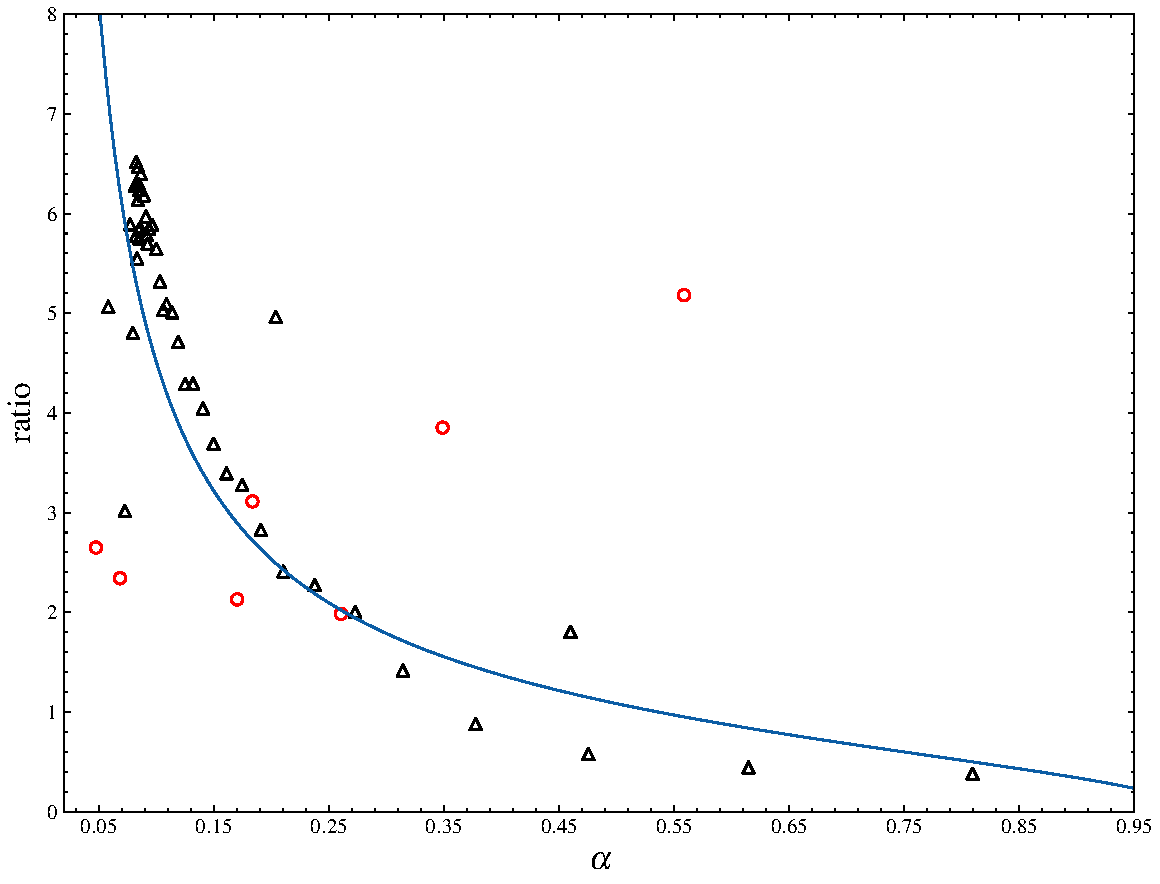
\includegraphics[scale=0.5]{img/fig_adiabatic.pdf}
    \caption{The current ratio with respect to the inhomogeneous parameter $\alpha$. The scattered points denote the ratio and $\alpha$ at difference spatial locations obtained from the numerical simulation in ref. \cite{zheng2023b}. 
    The solid curve is the result from adiabatic approximation.
    }
    \label{fig.adiabatic}
\end{figure}

The temporospatial evolution of the nonlinear current only depends on the integral over the slowly varying scale $\mathcal{J}$, and an inhomogeneity parameter $\alpha$, defined in Eq. (\ref{eq.alp0.5}). 
The $\mathcal{J}$ integral can be solved further harnessing the adiabatic motion of the trapped particle along the magnetic field line, similar to the previous work \cite{summers2012}. While $m_\mathrm{spx}$ and $n_\mathrm{spx}$ can be numerical integrated from Eq. (\ref{eq.function}).
Note that, since the hole is aligned with the slowly varying wave packet,  $\Delta f$ also contributes a complex phase $\phi_a(s_i,t)$ which is the phase of the slowly varying wave packet $\phi_a \equiv \arg(a)$.
Thus, the current in Eq. (\ref{eq.adi_J}) is proportional to $(m_\mathrm{s p x}+\imath ~ n_\mathrm{s p x}) \exp({\imath \phi_a(s_i,t)})$.
Now we can show the validity of the adiabatic approximation by examining the ratio of the imaginary and real component of $j_p$, i.e., $\mathrm{real}(j_p)/\mathrm{imag}(j_p)$.
The current ratio as function of $\alpha$ is shown in Fig. \ref{fig.adiabatic}.
Also, base on the above-mentioned Vlasov theory, we performed a corresponding numerical simulation \cite{zheng2023b}, in which the current is obtained directly from Eq. (\ref{eq.nonlinear_J}).
The corresponding $\alpha$ is obtained from the definition in Eq. (\ref{eq.alp0.5}) using the simulation data.
From Fig. \ref{fig.adiabatic}, we can find that the simulation results in a wide spatial range from the magnetic equator to the high latitude region (triangle shape) well agree with the adiabatic approximation.
While near the equator region (circle shape), the adiabatic approximation ceases to be valid. 
This indicates a rapid variation of the phase space in the equator region, which is related to the generation of the nonlinear chorus wave.

\section{Conclusion}
\label{sec:conc}
In this paper, we explore the dynamics of resonant electrons and the evolution of whistler chorus wave within the Earth's inner magnetosphere, focusing on the scale separation of electron motion and fast wave interaction.
We developed a Hamiltonian theory describes the dynamics of the resonant particles on the reference frame moving with the local resonance.
The slowly varying motion along the weakly inhomogeneous magnetic field and the fast varying wave-particle interaction can be separately managed.
Our work also provides several new view angle for the chorus chirping problem.
In the onset stage of the chorus chirping, our theoretical description can be greatly reduced, which is beneficial to compose of numerical solver without losing any key physics for the generation mechanism of the chorus emission.  
The discussed adiabatic regime also shows the potential chirping behavior with respect to the inhomogeneity parameter $\alpha$.


%\bibliographystyle{unsrt}
\bibliography{ref.bib}
\end{document}
